\documentclass[letterpaper, 12pt]{article}
\usepackage{longtable, tabu, amsmath, amssymb, mathrsfs, graphicx, natbib}
\setlength{\parskip}{.5cm plus4mm minus3mm}

\begin{document}

\title{Price indices for improved analytics and dynamic pricing in the event ticketing industry}
\author{\emph{Rohit Patel}\thanks{Kellogg School of Management}}
\date {March 6, 2016}
\maketitle
\begin{abstract} As dynamic pricing becomes more common for event tickets including NFL, MLB, NBA and NCAA games, the ability to effectively measure and track prices changes for an event over time becomes critical. Standard price measures that are currently used for price measurement are ill suited to capture the complexities of an event ticket. This article outlines new industry-specific measures for event tickets that enable lifecycle trend analysis for ticket prices and pricing analysis across events and across competitive intermediary platforms. The measures introduced are designed to be invariant under large ticket sales, volume changes, dealer behavior, and differences in seat values. Additionally, we discuss several factors affecting ticket prices that should be taken into account while implementing a dynamic pricing engine by ticket sellers.
\end{abstract}

\section{Introduction}
The adoption of dynamic pricing has accelerated across all the major sports leagues in the past few years. This has translated into improved attendance and higher revenues for the ticket sellers. With the increasing deman

Analytics on pricing the ticketing industry is at a nascent stage, and much of the analysis is done using average ticket prices or standard pricing measures that are often ill suited to capture the complexities of an event ticket. Even for a particular event at a particular time, no two tickets are identical, and better analyzing ticket prices requires more specific measures suitable for the analysis. This issue becomes more important in the world where dynamic pricing is increasing. Setting dynamic prices without \cite{rishe2003ticket} explore cross-sectional differences in ticket prices across teams and causes for the size and direction of seasonal price increases in the National Football League (NFL) based on data from 1996-2001, using average ticket price as the measure. Yet, events are played at different  \cite{price2003demand} develop a predictive model which includes game, team and university specific factors that are likely to influence game day demand for Division 1-A college football. \cite{coates2007ticket} explore the demand for attendance at professional sporting events using a data set that includes ticket prices and a price index reflecting prices for ancillary goods associated with attendance, and conclude that the attendance demand is price inelastic. In contrast to the exiting research, we look at the two sided market from an intermediary prospective, and aim to develop measures that enable comparisons with competing platforms. 

In many cases, suitable measures are not available to capture the phenomenon exhibited by ticket prices. This document aims to bridge the gap, in part, by introducing new statistical measures that possess certain desirable statistical properties, such as invariability under volume changes or ticket sales, dealer behavior, differences in seat values etc. We discuss how the measures developed are an improvement over the exiting ones in the literature, where applicable. We start with a qualitative discussion around the various considerations in pricing in Section~\ref{cip}. In Section~\ref{lcm} we describe measure to capture the lifecycle trends in the ticket market. Section~\ref{prm} introduces new pricing measures fit for comparison of ticket selling intermediary platforms. Throughout the paper, we refer to the intermediary and the intermediary platform interchangeably as $\mathcal{I}_0$.

At this point, we turn our attention to a set of measures that can be used to study the lifecycle patterns among events. 
\section{Lifecycle Analysis Measures}\label{lcm}
In Section~\ref{cip} we discussed how ticket demand varies over the lifecycle of an event ticket sales. Generally, different events exhibit different curve patters for sales, and an analysis of this trend and the ability to predict it can be greatly useful to setting ticket prices effectively and dynamically. In this section we discuss measures that aim to summarize the phenomenon in order to enable comparison and analysis across events. For each event, we will calculate the measure as follows:

\noindent Let

\noindent $t_p$ - Date when the primary sale opens\\
$t_r$ - Date when the resale market opens\\
$t_f$ - Date of the event\\ 

We divide the time period into deciles and mark the date that stands in the middle of resale and event date, $t_m = \frac{t_r+t_f}{2}$. For each decile, let $C(d)$ denote the total number of ticket sales in the $dth$ decile and $V(d)$ the total number of revenue in that decile for that event. Define:

\begin{align*}
	c(d) &= \frac{C(d)}{\sum_{i=1}^{10}C(i)}&\text{The proportion of sale (\# tickets) in a decile}\\
	v(d) &= \frac{V(d)}{\sum_{i=1}^{10}V(i)}&\text{The proportion of sale (GTV) in a decile}
\end{align*}

\noindent For each event calculate:
\begin{align*}
	&&M_c(e) &= \frac{1}{4}\left[\left\{\sum_{i=1}^{10} \left| \max(|i-5|,|i-6|) \cdot c(i) \right|\right\} -1 \right]\\
	or&&M_c(e) &= \frac{1}{4}\left[\left\{\sum_{i=1}^{5} \left[ (6-i) \cdot c(i) \right] +\sum_{i=6}^{10} \left[ (i-5) \cdot c(i) \right]\right\} -1 \right]
\end{align*}
And,
\begin{align*}
	&&M_v(e) &= \frac{1}{4}\left[\left\{\sum_{i=1}^{5} \left[ (6-i) \cdot v(i) \right] +\sum_{i=6}^{10} \left[ (i-5) \cdot v(i) \right]\right\} -1 \right]
\end{align*}
And,
\begin{align*}
	M'_c(e) &= \frac{1}{5}\left[\sum_{i=1}^{5} \left[ (i-6) \cdot c(i) \right] +\sum_{i=6}^{10} \left[ (i-5) \cdot c(i) \right]\right]\\
	M'_v(e) &= \frac{1}{5}\left[\sum_{i=1}^{5} \left[ (i-6) \cdot v(i) \right] +\sum_{i=6}^{10} \left[ (i-5) \cdot v(i) \right]\right]
\end{align*}

The measures work together to enable us to understand the trend. $M_c(e)$ varies between zero and one, where a value of zero signifies that all the sales are concentrated in the $5^{th}$ and the $6^{th}$ deciles, rather than earlier or later in the lifecycle. A value of one signifies the sales were concentrated entirely in the first or the last deciles. In practice, the extreme values of 0 or 1 are unlikely, since the sales are often spread over the entire period, and the measure is helpful in determining the level of concentration to which they are concentrated towards the ends. $M_v(e)$ is similar to $M_c(e)$ but provides an understanding of the gross ticket value - sales in terms of their value.

$M'_c(e)$ on the other hand is designed to capture the trend in sales towards earlier or later in the lifecycle. The range of values is between zero and one, and a value of one implies that all the sales were in the last decile, whereas a value of one means that all the sales were in the first decile. 

We will now discuss some measures for effectively understanding trends in prices across events and competitive platforms. 
\section{Price Index}\label{prm}
\cite{paasche1874preisentwicklung} and \cite{laspeyres1871ix} price indices are commonplace in literature for analyzing price trends, and related improvements proposed by Fisher index and Marshall-Edgeworth serve well in many situations. However, due to a changing inventory and the fact that the same seat is never sold twice for an event, these indices cannot readily be used. A usage based on average prices is often an imperfect solution (e.g. \cite{tremblaynfl} discuss prices using the Laspeyres index). This approach however masks the problem of changing inventory, and the quality of seats that might cause the price index to change despite constant prices or worse, prices moving in the opposite direction to the index. We try to solve the problem by internally weighing the prices by quantities to arrive at a daily index. However, since the quantities are changing and so is the quality of seats, we establish a baseline in order to use them in the index. This is akin to the Marshall-Edgeworth improvement, however we use baseline weighted values rather than a simple mean.

Let there be only one event. Let $p(l,d)$ and $q(l,d)$ be the price and quantity of a listing $l$ on date $d$. Let $D_b$ be defined as the `base period' - a date range over which base is calculate. Base is:

\begin{align*}
	p^*_s &= \frac{\sum_{l\in s, d\in D_b} p(l,d)\cdot q(l,d)}{\sum_{l\in s, d\in D_b} q(l,d)} \\
	q^*_s &= \frac{\sum_{l\in s, d\in D_b} q(l,d)}{\sum_{d\in D_b} 1} 
\end{align*}

For each section, a daily index is:
\begin{align*}
	p_{d,s} &= \frac{\sum_{l\in s} p(l,d)\cdot q(l,d)}{\sum_{l\in s} q(l,d)}\\
	q_{d,s} &= \sum_{l\in s} q(l,d)
\end{align*}

The price index for the day for the event is:

\begin{align*}
	P_d &=  \frac{\sum_{s\in S} p_{d,s}\cdot q^*_s}{\sum_{s\in S} q^*_s\cdot \pmb{1}_{[q_{d,s} > 0]} }\\
	Q_d &= \sum_{s\in S} q_{d,s}
\end{align*}

The aggregated indexed price for that event is: $P^* = \frac{\sum_{d\in D}P_d\cdot Q_d}{\sum_{d\in D}Q_d}$ \\

The price index for each section level (level 1, level 2) etc can be calculated the same as that for the entire event, simply by replacing the set $S$ of all sections by the set $S_1$ of all the sections in level 1, for ex. We also introduce a measure for the relative inventory quality as:
\begin{align*}
	Q & = \sum_{s\in S} \left[\left( \left( \frac{q_{d,s}(\mathcal{I}_0)}{\sum_{s\in S}q_{d,s}(\mathcal{I}_0)} \right) -  \left( \frac{q_{d,s}(\mathcal{I}_1)}{\sum_{s\in S}q_{d,s}(\mathcal{I}_1)} \right)\right)\cdot \frac{p^*_s}{\sum_{s\in S}p^*_s}\right]\\
	Q & = \sum_{s\in S} \left[\left\{ \left( \frac{q_{d,s}(\mathcal{I}_0)}{Q_d(\mathcal{I}_0)} \right) -  \left( \frac{q_{d,s}(\mathcal{I}_1)}{Q_d(\mathcal{I}_1)}\right) \right\}\cdot \frac{p^*_s}{\sum_{s\in S}p^*_s}\right]
\end{align*}

This measure compares the inventory quality between two platforms $\mathcal{I}_0$ and $\mathcal{I}_1$ by weighing the quantities of the tickets by a relative value measure. This value measure is calculated upon the base prices defined earlier.  




\section{Considerations In pricing}\label{cip}
Consider an intermediary $\mathcal{I}_0$ listing tickets on their online platform for sale. We discuss some of the factors and ticket price phenomenon that are exhibited by the ticket prices in the industry. While in no particular order, this discussion helps us better understand the dynamics in the industry and the motivation behind the statistical measures that are needed for analysis of competitive intermediary platforms.

\noindent {\bf Lifecycle Trends:} Ticket sales typically vary over the life cycle of the event, from the day the tickets are released for sale to the day of the event. Ticket resales over the lifecycle of the event are affected by:
\begin{itemize}\itemsep0em
	\item Date of resale market open
	\item Type of event (Sports fans typically purchase tickets late vs concert sales are concentrated to the beginning and end etc\dots
	\item Date to event 
	\item Weekday/holiday (sales on holidays are higher/lower etc.., this refers to the sale of a given event on the weekend, not the sales of events happening on the weekend)
\end{itemize}

\noindent {\bf Effective List Price:} There are multiple dynamics at play in determining the effective list price. For a given final checkout price, the list price can be set at a desired level using a combination of broker fees, buyer fees and markups. A lower list price seems to increase conversion at list, however, this increases the buyer fees which can have a different effect on the platform depending on buyer behavior
	\begin{itemize}\itemsep0em
		\item Buyer checks the seat on another platform for the same seat: In this case, if $\mathcal{I}_0$'s checkout price is lower, the buyer could either come back to complete the transaction or buy it from another platform due to inconvenience of multiple switches
		\item Buyer checks competitor for cheaper/more expensive seats: It is possible that a direct comparison does not happen, the buyer could think that he/she is getting a higher valued seat (judging by the list price) for a lower price, and might buy from the competing platform even though the ticket is a worse deal
	\end{itemize}
	These factors also have long term implication for $\mathcal{I}_0$. For example, a lower list price can make $\mathcal{I}_0$ appear to be a more competitive platform, however, the lower buying fees can make $\mathcal{I}_0$ seem like a platform with low fees and providing more valuable tickets for better price. Different customer segments can have different buying habits, for example, rare one-time buyers are more likely perhaps to be in a scenario where buyer fees are considered excessive because they have no objective sense of ticket value by looking at the list price. However, more seasoned players are more likely to select seats based on list price and then compare final checkout prices. Even more seasoned buyers can have the buyer fees built into their calculations. 

	Broker behavior can also play a factor in list price selection. Depending on broker behavior, different things can happen:
	\begin{itemize}\itemsep0em
		\item They simply add the amount to their desired take home
		\item They use a revenue maximizing strategy
		\item They actively manage list price
	\end{itemize}

\noindent{\bf Venue Size:} The size of the venue, given all other factors being the same, is expected to have a negative effect on ticket prices and a positive effect on the price elasticities. However, the venue size is more often than not correlated with other factors, complicating the efforts to isolate the effects of venue size:
\begin{itemize}\itemsep0em
	\item Venue size tends to be highly correlated with the stardom of the performer, this is a big factor when it comes to concerts. So while it can be assumed that the same star playing in a smaller venue will cause the price elasticities to be lower in comparison to them playing in a bigger venue - bigger starts typically tend to perform at bigger venues.
	\item Venue sizes also tend to be correlated with the location and population/demographic.
\end{itemize}

\noindent{\bf Stardom:} Stardom of the performers and players is one of the key determinants in ticket pricing. The effect is largely predictable. However, other confounding variables such as location or recency of performance can affect how the prices are impacted by stardom. For concerts, typically bigger stars cause the ticket prices to be higher given all other things being equal. When it comes to sports, a host of factors decide how stardom affects ticket prices and price elasticity. Stars can be a relatively more important factor for teams with traditionally less loyal fan base. Team recent performance and season performance are also factors that will impact the effect of stardom. Additionally, Stardom and performance of the opposing team is also a factor to consider for sports events.

\noindent{\bf Tiredness:} The frequency of the event for a particular team or performer is a factor in the ticket prices and elasticities. For example, if a band has it's only concert scheduled in a long time, a relatively modest fan base can be galvanized to drive up sales and reduce price elasticities.

\noindent{\bf Location:} The location of the event is a factor in determining the attractiveness. It affects in several ways:
\begin{itemize}\itemsep0em
	\item Star/Location fit, for example the home town/state of the star, or the home city of the team
	\item Population at the location and market size along with demographics
	\item Buying power at the location, average salary etc\dots
	\item Whether to location is a good tourist destination, since oftentimes fans will plan to visit the game along with a chance to visit the city
\end{itemize}

\noindent{\bf Competition Pricing:} The pricing of the competition affects the conversion rates, and in the long run, the ticket master platform popularity and market share. Key factors:
\begin{itemize}\itemsep0em
\item {\bf Reputation Effects:} $\mathcal{I}_0$'s pricing relative to the competition shapes the public opinion over a period of time. This can affect the percentage of the population that considers $\mathcal{I}_0$ as the go-to place for their buying and selling activities.
\item {\bf Conversion at List:} How much is conversion at list affected by the price relative to competition, and how does it play with revenue
\item {\bf Conversion at checkout:} It remains to be seen how the customers think or look at final checkout price and compare. Do they look at high fees and then go back to look at something cheaper on other platform, or the same ticket on other platform? At which point, if they see lower fees, but still higher checkout price, do they come back? What is the buying behavior here?
\end{itemize}

\noindent {\bf Broker Inventory Selection:} Brokers select the choice of their inventory, the scope of release and the timing. The selection is influenced by a myriad of factors. One key consideration is the need for brokers to manage market perception for the available tickets for a concert. Releasing limited inventory in order to limit the perceived number of available tickets can help create a feeling of scarcity in the mind of the fan, thus influencing their decision to buy the ticket sooner rather than later. Another consideration is that of competing platforms - brokers typically list tickets on multiple platforms depending on their fee structure and buyer and seller fees. This means sales on one platform requires a syncing of tickets on all platforms - something that can be expensive if done manually. Many brokers seek to avoid the problem by listing different inventory on different platforms.

\noindent{\bf Broker Sophistication and Dynamic Pricing:} The level of broker sophistication is a critical factor to be taken into account when determining price, and more importantly pricing dynamically. For example at any given point if the broker is assumed to be fully sophisticated and rational, they can change prices, taking into account the fees that will be charged by $\mathcal{I}_0$, to maintain the level of price that is optimal. As shown in Figure~\ref{fig:demc}, this level can be at an optimal level (for example, if the broker take is a \%) or suboptimal (for ex if the $\mathcal{I}_0$ take is a fixed fee). 
\begin{figure}[h]
	\centering
	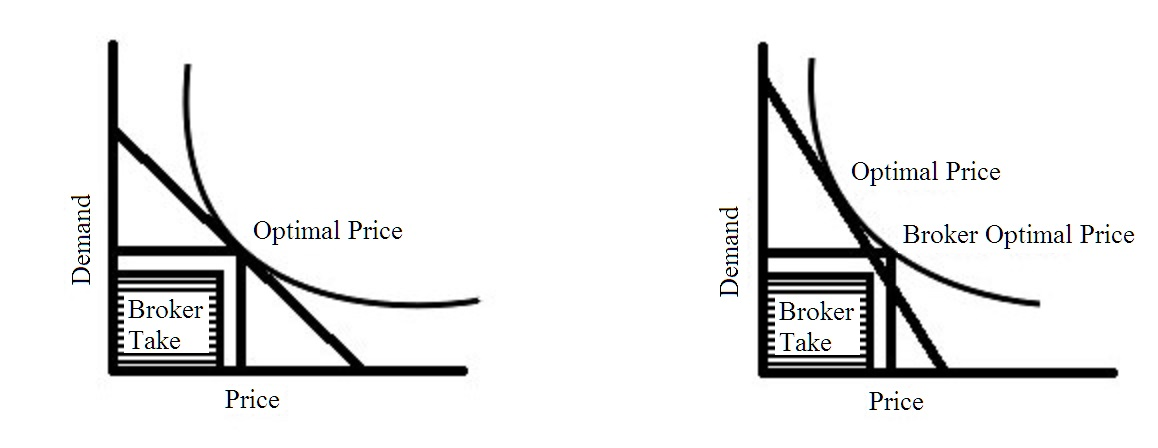
\includegraphics[scale=.3]{IMG_20151201_112640407.jpg}
	\caption{An optimal Pricing Choice for the Broker}
	\label{fig:demc}
\end{figure}

Furthermore, this directly affects the process of dynamic pricing. Consider Figure~\ref{fig:idp}; an illustrative optimal dynamic pricing schedule in the market. Now, this is typically unknown, and must be estimated with the help of certain variables. If $\mathcal{I}_0$ were the primary (and the only) player, then after estimating the price elasticities and then the optimal dynamic pricing schedule, a price schedule can be described. However, since the teams, and then the brokers, are doing their own determination of the optimal pricing schedule, $\mathcal{I}_0$ cannot simply set it's fees simply based on the estimated price elasticities. This type of pricing schedule adds on to the estimates (or wrong estimates) of the brokers and the teams, and is quite simply just as useful as a fixed price schedule. $\mathcal{I}_0$ needs to account for the strategies of the brokers and the competition in pricing to determine the optimal fee. 
\begin{figure}[h]
	\centering
	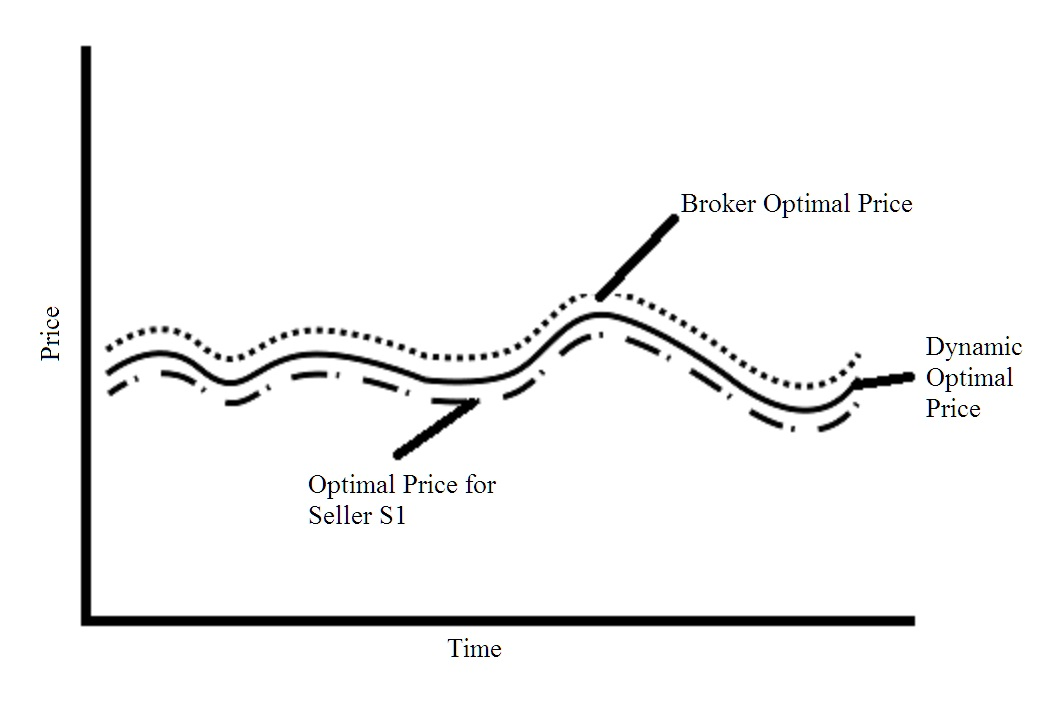
\includegraphics[scale=.3]{IMG_20151201_104645518.jpg}
	\caption{An ILLISTRATIVE Dynamic Pricing Schedule}
	\label{fig:idp}
\end{figure}





\section{Conclusion}
We have presented several measures that enable us to effectively capture the nuances of the ticketing industry, especially from the perspective of an intermediary. Moreover, we derived closed for expressions for impact on revenue from buyer an seller fee changes that are used to create an optimization engine for $\mathcal{I}_0$ to enable dynamic pricing. While derived in the context of a specific engagement, these tools add to the literature and can be used more generally to further investigate and improve efficiencies in the ticketing industry.

\bibliographystyle{aer}
\bibliography{ref}
\end{document}
